\chapter{Results \& Discussions}
\indent\indent This chapter provide details related to results of the design implementation. The results are divided as simulation result of 16 x 16 Vedic Multiplier using carry save adder and result of 16 x 16 Vedic Multiplier using high-speed area efficient adder.


\section{Simulation Result}
The simulation analysis of the 16 x 16 Vedic Multiplier using carry save adder and of 16 x 16 Vedic Multiplier using high-speed area efficient adder is carried out using Xilinx ISE Software. The simulation result is shown in Fig. \ref{fig:x7}.\\
\begin{figure}[htb]
	\centering
	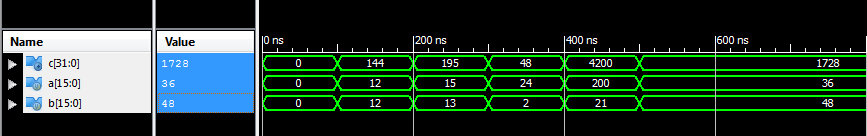
\includegraphics[width=0.9\columnwidth]{Figures/x7}	
	\caption{Simulation Result of 16 x 16 Vedic Multiplier}
	\label{fig:x7}
\end{figure}
Here A \& B are the input 16-bit data and C is the 32 bit multiplier output. One can easily observe that the output for 16 x 16 Vedic Multiplier using carry save adder and 16 x 16 Vedic Multiplier using high-speed area efficient adder has been obtained successfully. The multiplication of 21 \& 200 yields 4200 and multiplication of 13 \& 15 yields 195, simlarly the other multiplication input combinations can be observed and the results are true with no errors.
\begin{table}[htb]
\fontsize{10}{12}\selectfont
\caption{Comparision of Critical Path Delay and Total Power}
\label{tab:tab1}
\centering
\begin{tabular}{@{}|c|c|c|c|@{}}
\toprule
\textbf{SL NO} & \textbf{\begin{tabular}[c]{@{}c@{}}16x16 Vedic Multiplier\\ using\end{tabular}} & \textbf{\begin{tabular}[c]{@{}c@{}}Critical Path\\ Delay(ns)\end{tabular}} & \textbf{\begin{tabular}[c]{@{}c@{}}Total Power \\ (µW)\end{tabular}} \\ \midrule
1              & \textbf{CSA}                                                                    & 0.882                                                                 & 70                                                                   \\ \midrule
2              & \textbf{HSAE Adder}                                                             & 0.824                                                                 & 55                                                                   \\ \bottomrule
\end{tabular}
\end{table}
From the table \ref{tab:tab1} we can observe the results that the 16x16 Vedic Multiplier using High-speed-area-efficient adder is having the total power and critical path delay of 55µW and 824ps respectively which is much better as compared to 16x16 Vedic Multiplier using CSA.




